\section{Introduction} \label{sec:intro}



\section{The Faro Framework} \label{sec:faro}

\faro has adopted a modular and extensible design that can be configured  to run any subset of metrics on any subset of data products, e.g., a  subset of the realtime metrics computed on a single exposure. 
Two main components form the basis of the \faro framework;  a collection of \texttt{Task}s that compute specific metric values, and a set of base classes that handle data i/o for various types of input data units corresponding to the granularity of metric computation, e.g., per-detector, per-visit, per-patch, per-tract. 
\faro builds upon much of the existing infrastructure of the LSST Science Pipelines, in particular the ``Generation 3'' middleware, including the Data Butler and Task Framework\footnote{\url{https://pipelines.lsst.io/modules/lsst.pipe.base/task-framework-overview.html}}\cite{dmtn-229}, and the LSST verification framework\cite{SQR-019}. 
The LSST Data Butler (hereafter the ``Butler'') provides an abstracted data access interface that is used to read and write data without having to know the details of file formats or locations.
The Butler organizes data, both raw and processed, into data repositories.
A \texttt{Task} is a reusable unit of code in the LSST science pipelines infrastructure that is used to process data.
Each Task has a specialized configuration object attached to it and provides a \texttt{run()} method that implements the algorithm to execute. 
Each \faro metric has an associated \texttt{Task} class that implements the mathematical algorithm to compute the scalar metric value on the input data.
The LSST Verification Framework, \texttt{lsst.verify}, is a framework for making verification measurements in the LSST Science Pipelines.
\faro takes as input catalog data products generated by the LSST Science Pipelines\footnote{The LSST science pipelines produce catalog data products both in FITS and parquet file format. \faro works exclusively with with parquet formatted data.} stored in a Butler repository, 
%  but in principle could use any data product available in a Butler repository, including images, 
 and computes scalar performance metrics on them. 
The resulting metric values
% \footnote{The result of computing a given metric on some set dataset.} 
are persisted in the same Butler repository alongside the input data products, each with an associated searchable data identifier\footnote{A dict-like identifier for data usable across multiple Butler collections and DatasetTypes.} as \texttt{lsst.verify.Measurement} objects.

\subsection{Analysis Contexts} \label{ssec:analysis_context}

An analysis context defines the type of input data unit corresponding to the granularity of metric computation, e.g per-detector, per-visit, per-patch or per-tract.
\faro supports metric calculation for a multiple analysis contexts, that is, the same mathematical function can be called in a different analysis context to produce a different metric value. 
For example, the photometric and astrometric repeatability metrics,  and  band-to-band astrometric transformation accuracy metrics are computed  at the visit level on single-frame data products, whereas  residual PSF ellipticity correlation metrics could be computed at either a per-visit level or on a per-tract level on the coadded data products
For some metrics, only certain analysis contexts make sense and often the choice of analysis context will be dictated by statistics, e.g a small 1\degsq CI dataset may not contain enough data to compute some metrics on a per-tract level. 
\faro allows users to easily define a new analysis contexts for their particular science need. 

The following analysis, corresponding to analysis contexts  are currently supported in \faro:
\begin{itemize}
\item per-detector source catalogs i.e., single-visit detectionsThanks.
\item per-visit source catalogs i.e., single-visit detections
\item per-patch object catalogs i.e., coadd detections both per-band and multi-band
\item per-tract object catalogs i.e., coadd detections, both per-band and multi-band input
\item per-patch matched source catalogs, i.e., set of single-visit detections of the same objects, both single band and multi-band input
\item per-tract matched source catalogs, i.e., set of single-visit detections of the same objects 
\end{itemize}

\subsection{Base Classes} \label{ssec:base_classes}

\faro provides a set of base classes corresponding to the various analysis contexts described above that use the \texttt{PipelineTask} framework to build a quantum graph\footnote{A data structure that represents a concrete workflow generated from a Pipeline.} and interact with Butler for data i/o.
The base classes abstract away the data i/o, leaving the scientist free to focus on the algorithmic details  relevant to their particular analysis. 
The primary base classes in the lsst.faro package are \texttt{CatalogMeasurementBaseConnections}, to define the desired i/o,  \texttt{CatalogMeasurementBaseConfig}, to provide the configuration, and \texttt{CatalogMeasurementBaseTask}, to run the algorithm and store teh output data in the Butler. 
Each of these base classes inherits from \texttt{MetricConnections}, \texttt{MetricConfig}, and \texttt{MetricTask}, in the \texttt{lsst.verify} package respectively, and adds additional general functionality for computing science performance metrics based on Source and Object catalog inputs. 
Additional base classes can be easily added following this scheme for new analysis contexts. 

\subsection{Stages of Metric Computation} \label{ssec:stages}

Metric computation with \faro proceeds through three stages:
\begin{enumerate}
\item \textbf{Preparation:}  any intermediate data products that are needed as input to the subsequent measurement step are assembled and persisted in the Butler.	
\item \textbf{Measurement:} the metric \texttt{Task} is run to compute a measurement for each unit of data (i.e., a quantum of processing with a particular a dataId for the output measurement). Measurements are stored as \texttt{lsst.verify.Measurement} objects.
\item \textbf{Summary:}  a single scalar summary statistic, e.g a mean, median, etc is generated from the collection of input measurements computed in the measurement stage.  Summary statistics are stored as \texttt{lsst.verify.Measurement} objects and persisted in the Butler.
\end{enumerate}
Not all metrics will necessarily have a  preparation stage as there may be no additional intermediate data products needed to compute the metric than those generated as part of the pipelines processing, however all must have a measurement and summary stage. 

Take as an example the photometric repeatability metric, PA1, which measures the RMS photometric repeatability of bright non-saturated unresolved point sources in a single filter.
During the preparation stage, a matched source catalog is created for each tract and band that matches source detections in individual visits that correspond to the same physical astronomical object\footnote{LSST defines an Object as an astrophysical physical object, e.g a star, galaxy or asteroid, and a Source as a  single detection of an astrophysical object in an image. The association of Sources that are non-moving lead to Objects; the association of moving Sources leads to Solar System Objects.}. 
During the measurement stage, for each tract and band, the matched catalog computed and stored in the preparation stage is loaded into memory and used to compute the RMS scatter of fluxes for a single astrophysical object. 
In the final summary stage, the measurements for the ensemble of individual tracts computed in the measurement stage are loaded to compute a median summary statistic per band. 
This final summary statistic characterizes the overall performance for the dataset per band and is stored as an \texttt{lsst.verify} object in the Butler. 

\subsection{Processing Pipelines} \label{ssec:pipelines}

Pipelines, configurations in the form of YAML files, are used to define the \faro metrics to be computed together with the  detailed execution parameters for metric calculations. 
The \faro package provides a set of pre-defined pipelines, defined per analysis context, for many common configurations of computing metrics. 
\faro pipelines can be run as an after burner to the LSST Science Pipelines or can be interspersed with science pipelines processing to compute , as long as the necessary input data products have been computed and are stored in the Butler.  
For example, all single-visit metrics can already be computed once the single-frame processing steps have completed. 
This enables us to promptly assess performance and take any corrective action early. 
Figure \ref{fig:faro_pipeline} shows an example of a \faro pipeline describing the measurement stage of the computation of three performance metrics  using a per-tract matched catalog analysis context.
Pipelines can be built hierarchically, with a high-level pipeline calling lower-level pipelines, as shown in figure \ref{fig:faro_pipeline_hierarchy}.

\begin{figure}[!ht]
  \lstset{language=YAML}
  \begin{lstlisting}
description: Compute metrics from matched catalogs
tasks:
  PA1:
    class: lsst.faro.measurement.TractMatchedMeasurementTask
    config:
      connections.package: validate_drp
      connections.metric: PA1
      python: |
        from lsst.faro.measurement import PA1Task
        config.measure.retarget(PA1Task)
  PF1_design:
    class: lsst.faro.measurement.TractMatchedMeasurementTask
    config:
      connections.package: validate_drp
      connections.metric: PF1_design_gri
      python: |
        from lsst.faro.measurement import PF1Task
        config.measure.retarget(PF1Task)
        config.measure.threshPA2 = 15.0
    \end{lstlisting}
  \caption{A \faro pipeline describing the measurement stage of the computation of three performance metrics per-tract from matched catalogs.}
  \label{fig:faro_pipeline}
\end{figure}

\begin{figure}[!ht]
  \lstset{language=YAML}
  \begin{lstlisting}
description: Complete metrics measurement pipeline
imports:
  # Photometric and astrometric repeatability:
  - location: $FARO_DIR/pipelines/metrics_pipeline_matched.yaml
  # Astrometry relative to a reference band:
  - location: $FARO_DIR/pipelines/metrics_pipeline_matched_multi.yaml
  # Ellipticity residual correlations, visit-level:
  - location: $FARO_DIR/pipelines/metrics_pipeline_visit.yaml
  # Ellipticity residual correlations, coadds:
  - location: $FARO_DIR/pipelines/metrics_pipeline_tract.yaml
  # Stellar locus width:
  - location: $FARO_DIR/pipelines/metrics_pipeline_tract_multi.yaml
    \end{lstlisting}
  \caption{A \faro pipeline showing how pipelines for pre-defined groups of metrics can be called hierarchically.}
  \label{fig:faro_pipeline_hierarchy}
\end{figure}

\section{Adding a  Metric} \label{sec:add}

We anticipate that many developers and scientists will want to define write their own metrics specifically to address concerns that arise as LSST progresses through the construction phase and into operations.
The first step in writing a new metric is to define the analysis context (\S \ref{ssec:analysis_context}) and to review the associated \texttt{Connections},  \texttt{Config}, and  \texttt{Task} base classes (\S \ref{ssec:base_classes}) to understand the in-memory python objects that will be passed to the run method of the metric measurement task, and the configuration options.
If the required analysis context and associated base class do not exist, they must first be created. 
Once the analysis context and base class are defined, the metric can be implemented by creating a measurement \texttt{Task}, an instance of \texttt{lsst.pipe.base.Task} that will operate on in-memory python objects and compute the metric. 
Finally, the new metric is added to the appropriate pipeline YAML file so that it can be run.
Figures \ref{fig:num_sources_task} show an example of a non-normative metric \texttt{Task} written to compute the number of rows in an input Source or Object catalog, \texttt{NumSourcesTask}

\begin{figure}[!htp]
  \lstset{language=python}
  \begin{lstlisting}
  
class NumSourcesTask(Task):

    ConfigClass = NumSourcesConfig
    _DefaultName = "numSourcesTask"

    def run(self, metricName, catalog, **kwargs):
        self.log.info("Measuring %s", metricName)
        if self.config.doPrimary:
            nSources = np.sum(catalog[self.config._getColumnName(
                "detect_isPrimary")] is True)
        else:
            nSources = len(catalog)
        self.log.info("Number of sources (nSources) = %i" % nSources)
        meas = Measurement("nsrcMeas", nSources * u.count)
        return Struct(measurement=meas)    \end{lstlisting}
        
  \caption{Implementation of a simple task to count the number of Sources or Objects in an input catalog. }
  \label{fig:num_sources_task}
  \par\medskip
\end{figure}

\section{Tracking and Visualization} \label{sec:tracking}

We visualise and track the time evolution of \faro metrics using the LSST metrics dashboard, \squash\cite{SQR-009}. 
\squash makes use of the InfluxDB\footnote{\url{https://www.influxdata.com/}} time series database as the backend store for time-stamped metrics and the Chronograf\footnote{\url{https://www.influxdata.com/time-series-platform/chronograf/}} user interface.
InfluxDB is designed to store large volumes of time series data and quickly perform real-time analysis on that data.
Chronograf provides dashboards to easily visualise and track metrics stored in InfluxDB. 
Metrics computed by \faro on the outputs of the LSST Science Pipelines are stored in the Butler and then pushed to the \squash using  the InfluxDB REST AP
From the Chronograf UI, the user can query the metric values, aggregate results and create alerts when measured metrics change or go out of specification. 
By tracking metric measurements we are able to understand trends in the algorithmic performance of the LSST Science Pipelines, and ultimately verify that we will meet our requirements.
We have configured a number of dashboards for tracking \faro metics computed on various precursor datasets at different cadences, e.g nightly, monthly, etc. 
Figure \ref{fig:squash_metrics_ci} shows the dashboard for \faro metrics computed on the nightly CI dataset (\S \ref{sssec:ci}). 
\begin{figure}[!htp]
  \par\medskip 
  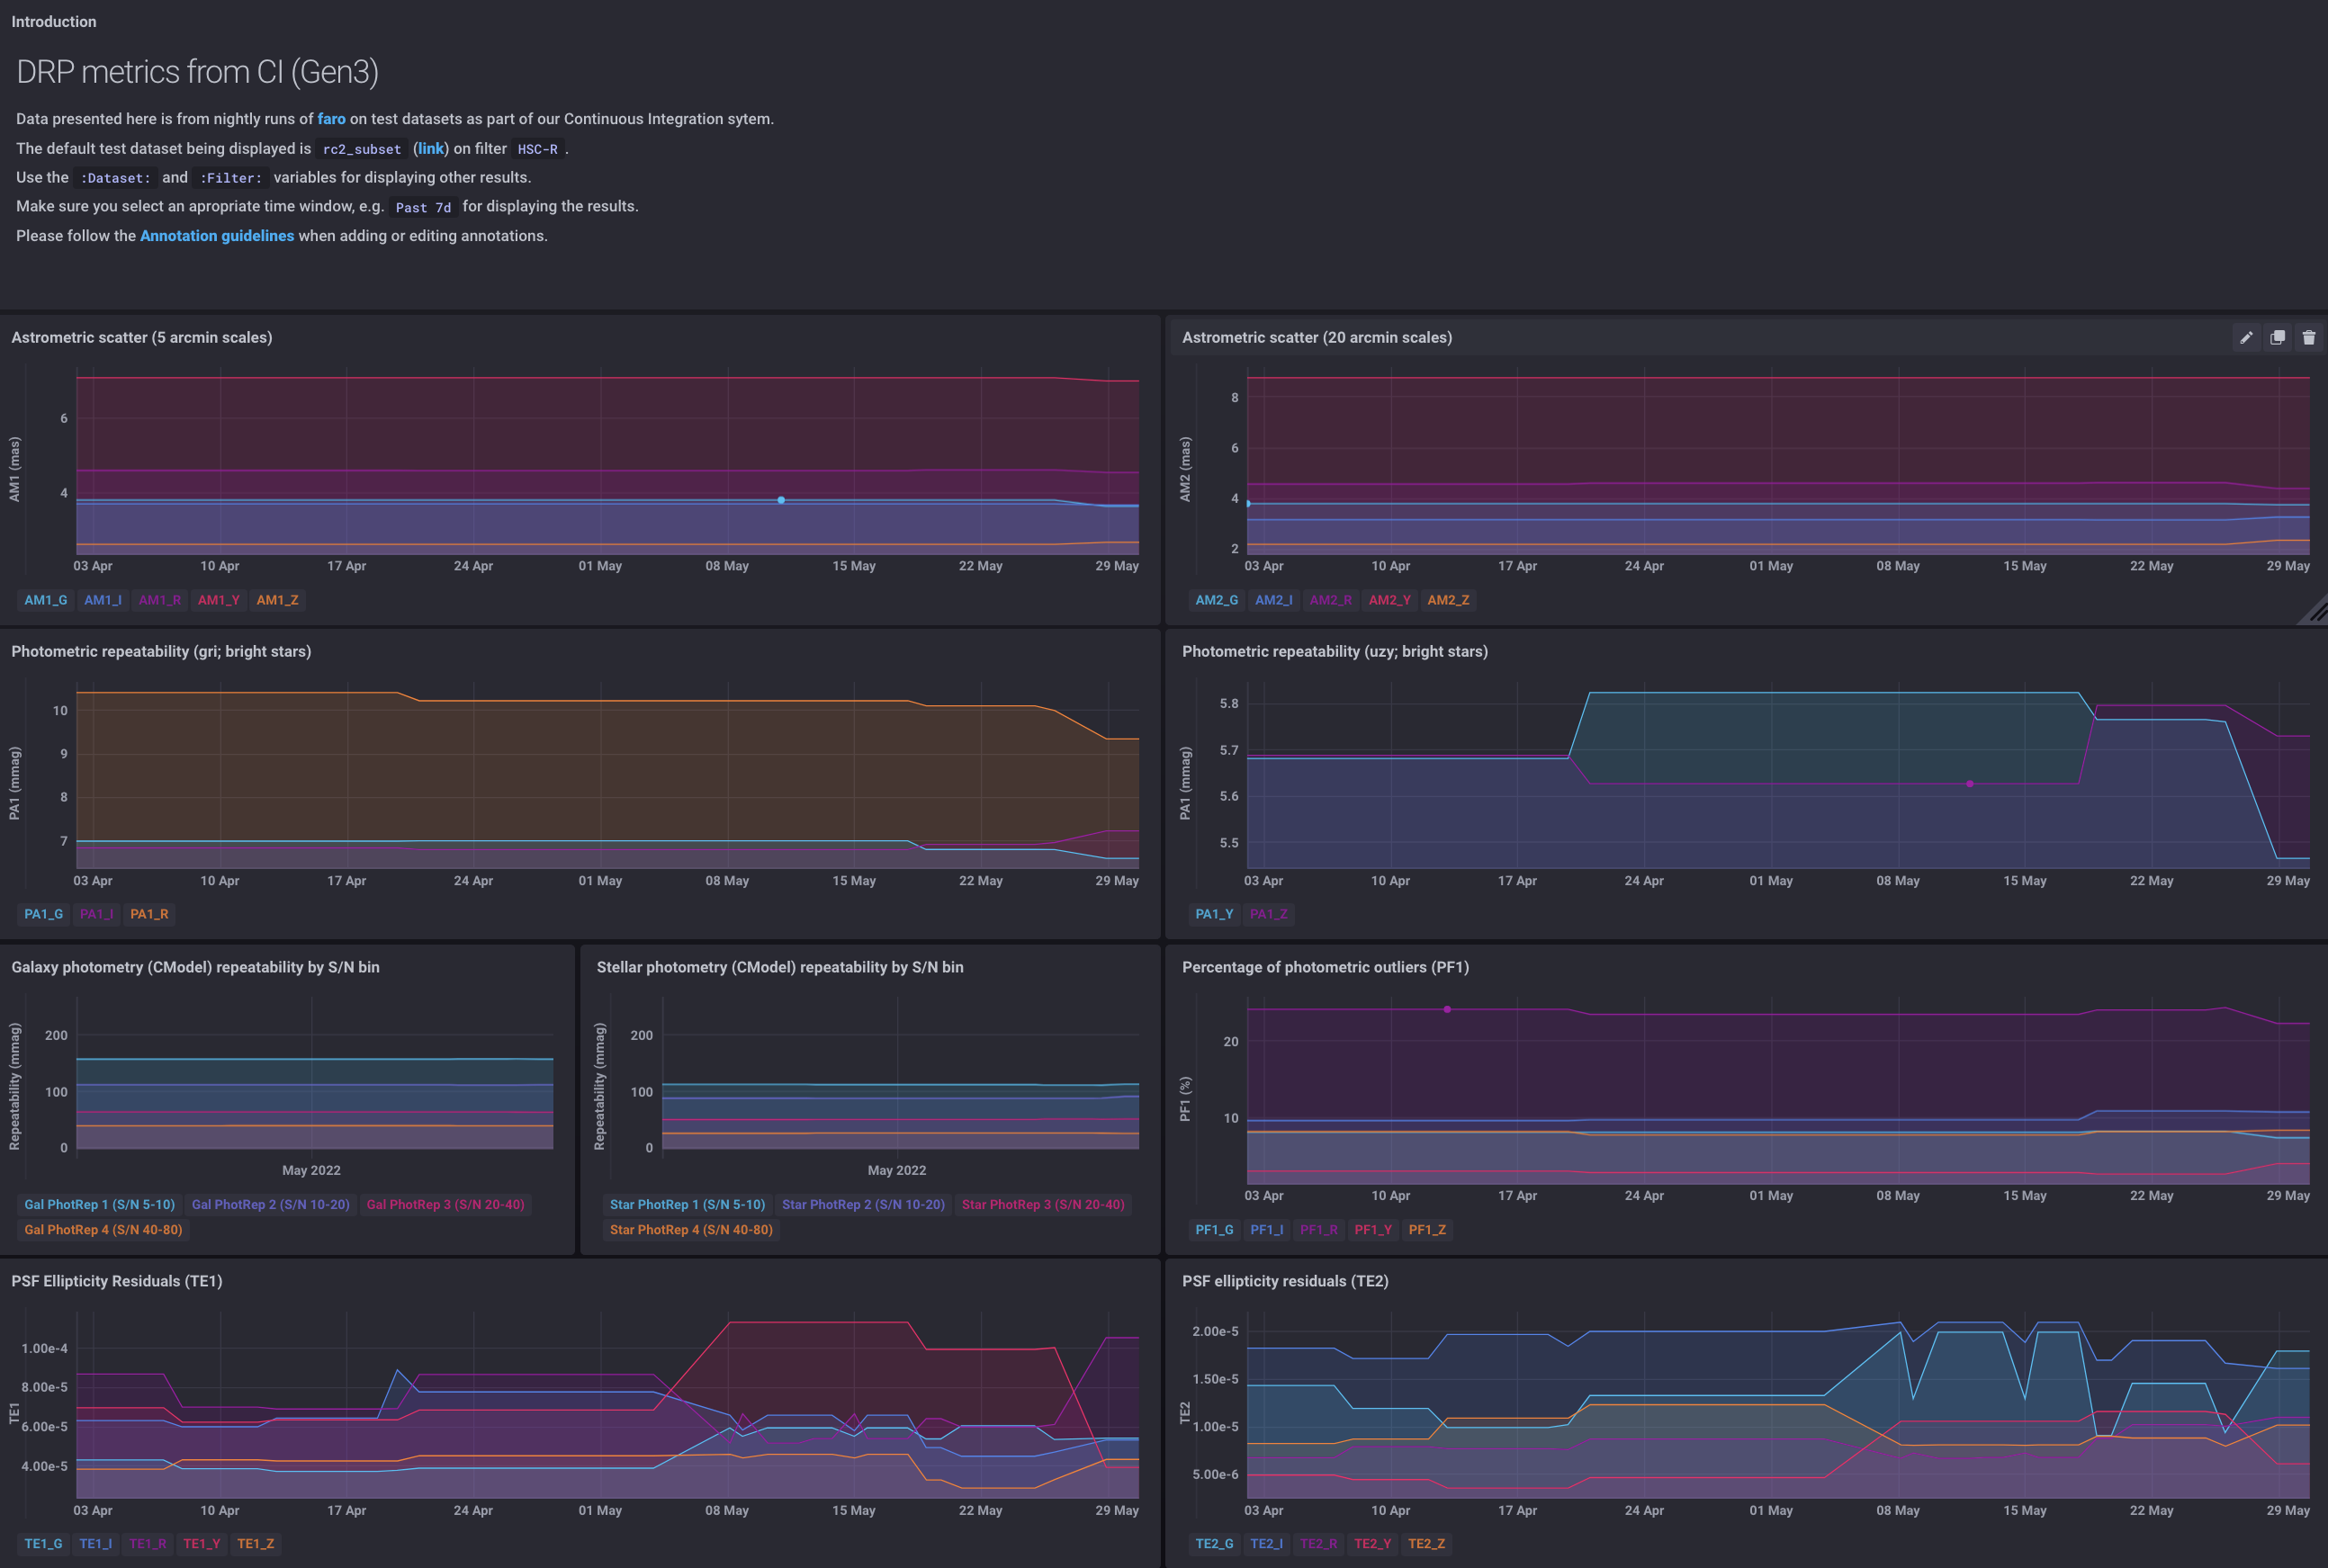
\includegraphics[width=0.98\textwidth]{figures/squash-dashboard-ci.png}
  \par\medskip   
  \caption{InfluxDB/Chronograph dashboard}
  \label{fig:squash_metrics_ci}
\end{figure}


\section{Faro Applications} \label{sec:applications}

\subsection{Monitoring Science Pipelines Performance} \label{ssec:monitoring}

\faro is used to monitor the scientific performance of the LSST science pipelines on precursor datasets of different sizes and on a variety of cadences\cite{dmtn-091}. 
By tracking metrics computed on the outputs of evolving versions of the science pipelines using a fixed dataset we can rapidly identify the effect of code or configuration changes on the data products as development progresses during the LSST construction period.

\subsubsection{Continuous Integration}\label{sssec:ci}

The LSST Science pipelines are run nightly and weekly on a small subset of the Hyper Suprime-Camera (HSC) Release Candidate 2 (HSC RC2) dataset\footnote{\url{https://github.com/lsst-dm/rc2_subset}} in the LSST Jenkins-based continuous integration (CI) system. 
This datasets consists of the central 6 detectors for 8 randomly chosen visits in the 5 broad band filters in the HSC COSMOS field, and was produced specifically for measuring metrics in a CI environment.
\faro pipelines are run on the outputs in a per-visit or per-detector analysis context.
Given the small size of the dataset, there are not enough statistics to compute metrics on a per-tract level 
The goal is to track daily the performance of the pipelines, the quality of the data products, and to rapidly identify the effect of code or configuration changes on the data products as development progresses during the LSST construction period.
Figure \ref{fig:ci_metrics} shows an example of two metrics that are tracked and how they were used to identify the effect of a software change.
Metrics are reviewed regularly allowing us to identify changes and understand the impact of changes in the science pipelines.
\begin{figure}[!htp]
\begin{subfigure}{.5\textwidth}
    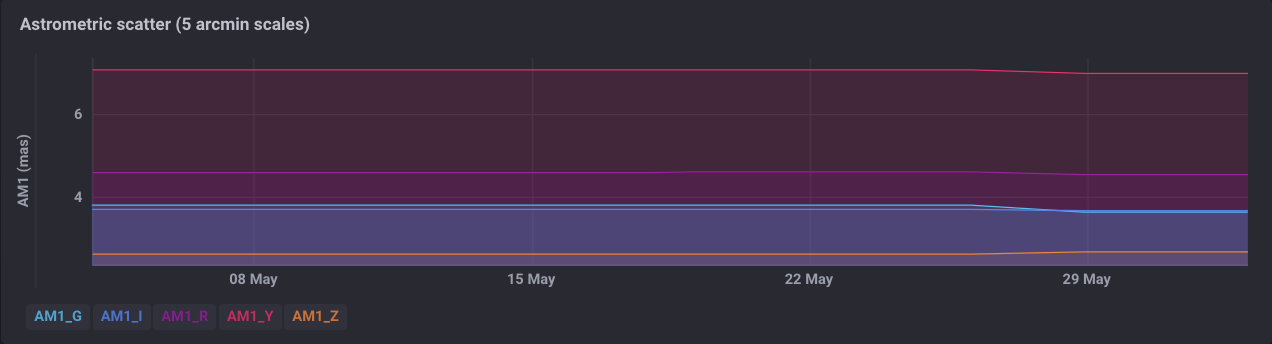
\includegraphics[width=0.98\textwidth]{figures/ci_metric_AM1_5}
\end{subfigure}%
\begin{subfigure}{.5\textwidth}
    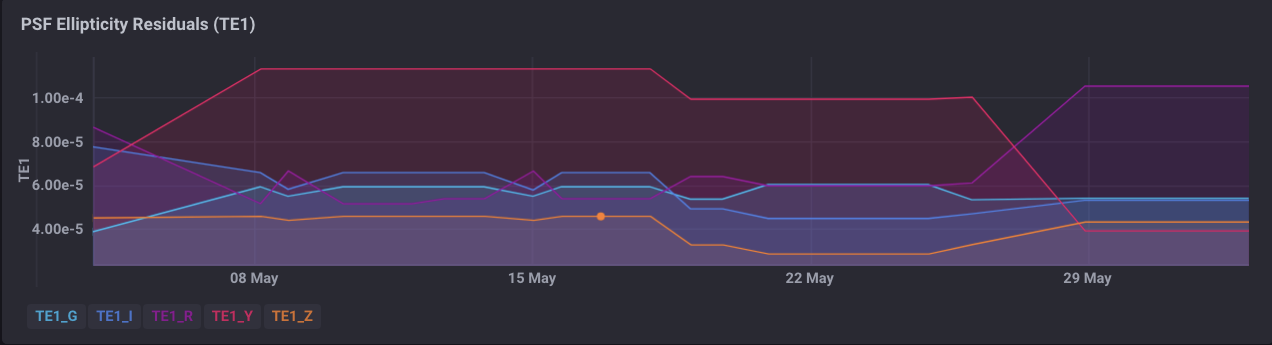
\includegraphics[width=0.98\textwidth]{figures/ci_metric_TE1}
\end{subfigure}
\par\medskip % force a bit of vertical whitespace
\begin{subfigure}{.5\textwidth}
    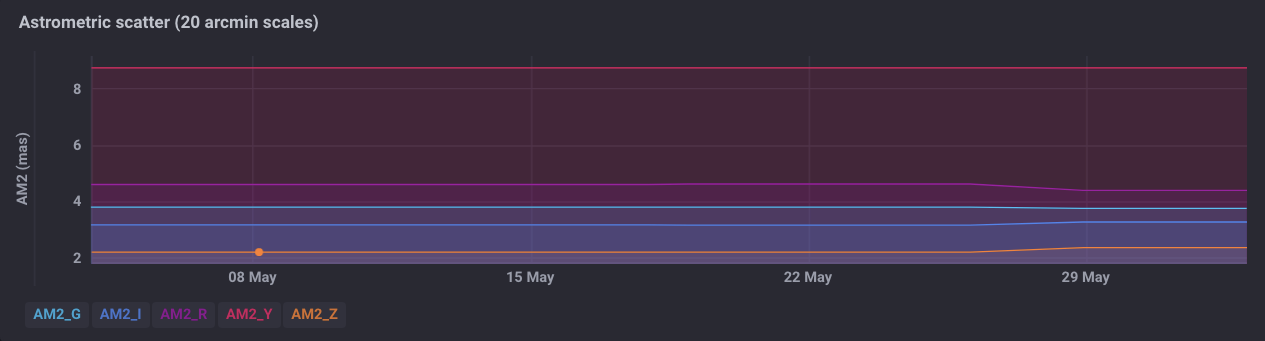
\includegraphics[width=0.98\textwidth]{figures/ci_metric_AM1_20}
     \caption[\small]{(a) Astrometric precision metrics}
\end{subfigure}%
\begin{subfigure}{.5\textwidth}
    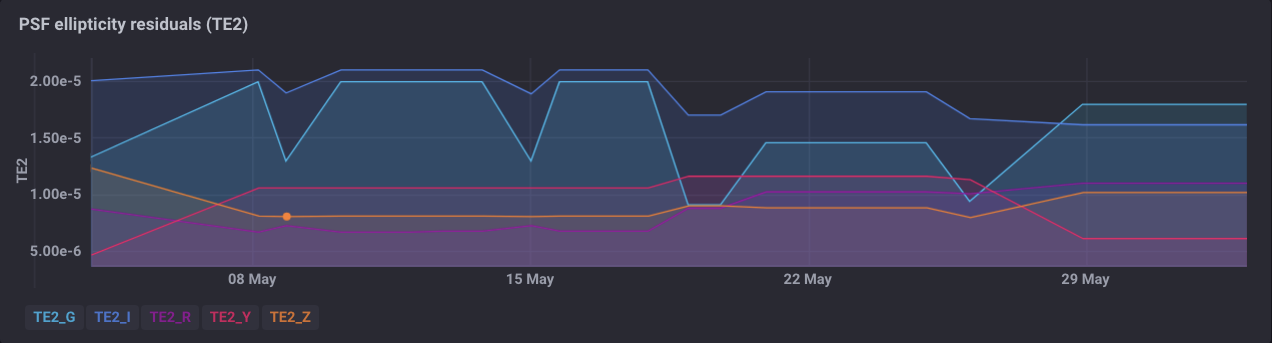
\includegraphics[width=0.98\textwidth]{figures/ci_metric_TE2}
    \caption[\small]{(b) Residual PSF ellipticity correlation metrics}
\end{subfigure}
\par\medskip % force a bit of vertical whitespace
\caption[short]{Examples of the time evolution of four \faro metrics computed on a nightly cadence in CI over a period of one month on the outputs of the nightly data release processing of a small subset of the HSC PDR2 dataset.  
Left shows the AM1 metric that characterizes the astrometric scatter on two different spatial scales, 5 and 20 arcmins, and right shows the residual PSF ellipticity correlations, TE1 and TE2. }
\label{fig:ci_metrics}
\end{figure}

\subsubsection{Software Release Characterization } \label{sssec:characterization}

Major releases of the LSST science pipelines are made approximately once every six months. 
Every major release is accompanied by a Characterization Metric Report, which describes the scientific performance of the release by computing \faro metrics on the full HSC RC2 dataset. 
HSC RC2 consists of 3 tracts of data taken and selected to provide a means of testing various pathological cases e.g., difficult astrometric solutions, extremely good seeing that does not provide a well-sampled PSF, difficult fields for deblending, and large galaxies, among others. 
These three tracts each contain between 112--149 visits split between the HSC-G, HSC-R, HSC-I, HSC-Z, and HSC-Y (grizy) filters.
The Characterization Metric Report compares values of metrics computed on the HSC RC2 dataset with a) those computed using the previous release of the science pipelines and b) the LSST SRD design specifications. 
This allows us to monitor the effects of major strategic developments in algorithms over longer periods of time. 
Figure \ref{fig:cmr_r23} shows an excerpt from the Characterization Metric Report \cite{dmtr-351} for the most recent release of the LSST science pipelines, Release 23.0.1.
From this excerpt, we see that there were improvements in the photometry and ellipticity correlation metrics as compared to the previous release, which reflect improvements in the photometric calibration algorithms to better handle fields of view near the spatial edges of survey footprints. 
\begin{figure}[!ht]
  \centering
  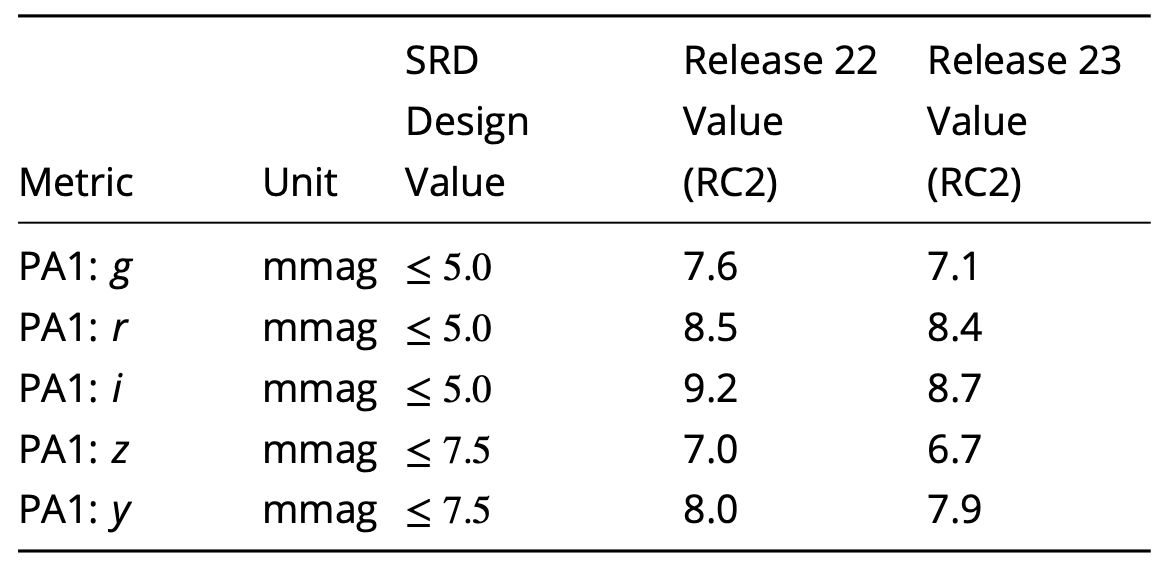
\includegraphics[width=0.45\textwidth]{figures/cmr_r23_photometric_metrics} 
  \hspace{0.5cm}
  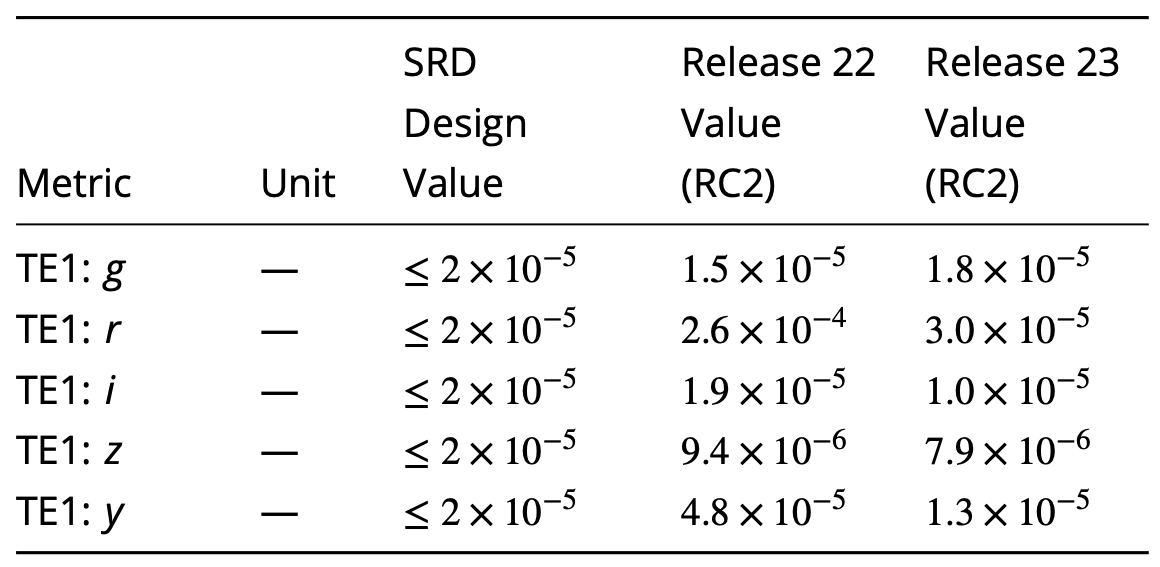
\includegraphics[width=0.45\textwidth]{figures/cmr_r23_ellipticity_metrics}
  \par\medskip % force a bit of vertical whitespace
  \caption{Excerpt from the  LSST Science Pipelines major Release 23 Characterization Metric Report on the HSC RC2 dataset. Metric values are compared with those of the previous release of the science pipelines and with the design specifications from the LSST Science Requirements document SRD.}
  \label{fig:cmr_r23}
\end{figure}

\subsection{Rubin Auxiliary Telescope Imaging Surveys} \label{ssec:auxtel}

The Rubin Auxiliary Telescope\cite{10.1117/12.2561112} (AuxTel) is a 1.2m f/18 telescope that sits adjacent to Rubin Observatory that will be measure atmospheric transmission using broadband spectroscopy of bright stars throughout survey operations. 
During the commissioning AuxTel is also being used as a data processing pathfinder via a series of imaging surveys.
The first AuxTel imaging campaign collected multiband data over a single field of high stellar density.
An average of 10 visits per pointing within the 1 \degsq survey single field were collected. 
The data was processed with LSST Science Pipelines, including measuring science performance metrics with \faro to provide near-realtime feedback to observers on the summit.
This dataset is than sufficient to explore coadds, repeatability and optimize processing configurations.
Single-visit science performance metrics including  were computed with \faro using data generated from the AuxTel Imaging Survey. 
Figure \ref{fig:faro_auxtel_metrics} shows some of the performance metrics computed with \faro as part of the AuxTel imaging survey

\begin{figure}[!ht]
\begin{subfigure}{.5\textwidth}
    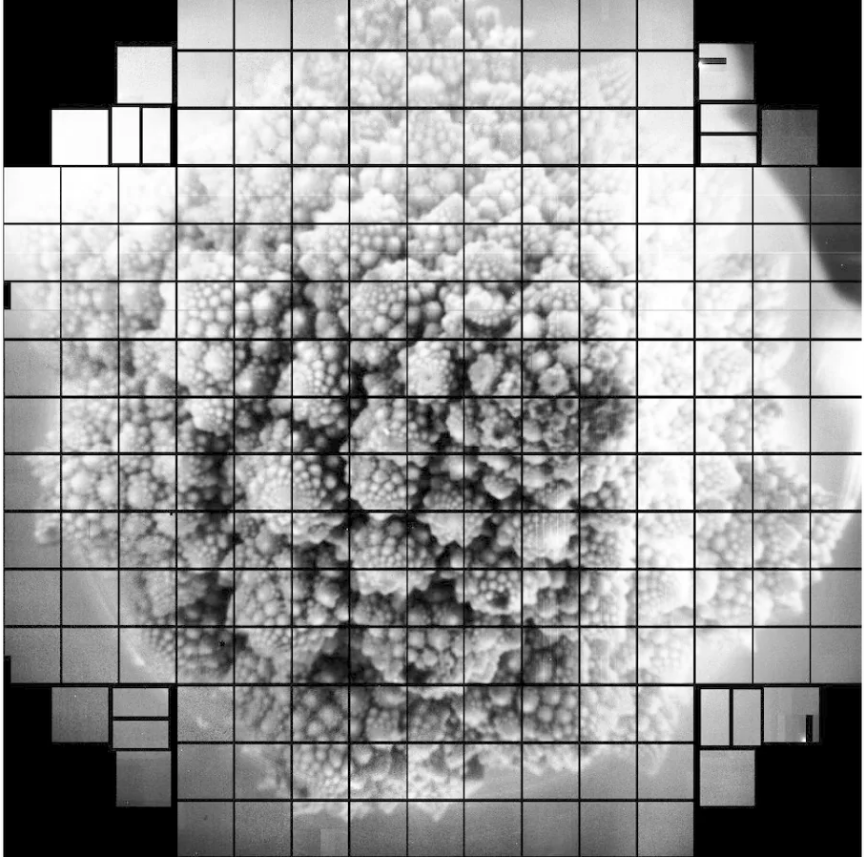
\includegraphics[width=0.8\textwidth]{figures/rubin_romanesco}
     \caption[\small]{(a) AuxTel metric }
\end{subfigure}%
\begin{subfigure}{.5\textwidth}
    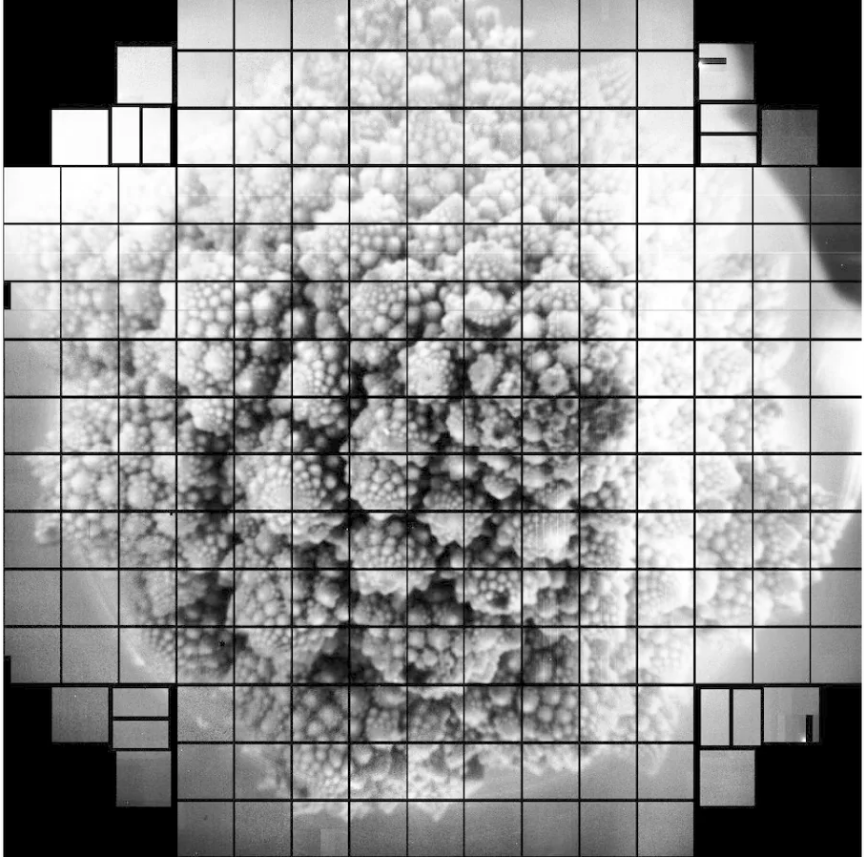
\includegraphics[width=0.8\textwidth]{figures/rubin_romanesco}
    \caption[\small]{(b) AuxTel metric}
\end{subfigure}
\par\medskip % force a bit of vertical whitespace
\caption[short]{\color{red}AuxTel metrics ---- Erik/Peter what would you put here}
\label{fig:faro_auxtel_metrics}
\end{figure}

\subsection{Rapid and first-look analysis} \label{ssec:rapid}

During LSST observing, early analysis of the images coming off the camera will be carried out on the mountain on the timescales of a few minutes. 
The following are examples of metrics that could be implemented in \faro to support this rapid first-look analysis:
\begin{itemize}
\item Number of detected Objects,
\item Sky brightness, counts and variance 
\item Image quality, specifically FWHM, PSF ellipticity
\item Comparison to reference catalogs, e.g Gaia to look for an excess/deficit of detections, astrometric offsets, photometric residuals or problems with PSF modelling,
\item Effective survey depth
\item Anomoly detection
\end{itemize}

\subsection{Rubin Data Previews} \label{ssec:datapreviews}

During the period leading up to the start of operations in 2024, Rubin Observatory will deliver a series of three Data Previews to the community. 
The goals of these Data Previews are twofold, to serve as an early integration test of the LSST Science Pipelines and the Rubin Science Platform (RSP)\footnote{A set of integrated web applications and services deployed at Rubin Data Access Centers (DACs) through which the scientific community will access, visualize, subset and perform next-to-the-data analysis of LSST Data products.} \cite{lse-319}, and to enable a limited number of scientists to begin early preparations for science with the LSST.
All  Rubin Data Previews are hosted at the Interim Data Facility (IDF) on Google cloud\cite{2021arXiv211115030O}.

Data Preview 0 (DP0) \cite{RTN-001} is the first of these three data previews.
The data set adopted for DP0 is the DESC 300 \degsq catalog of simulated LSST-like images and catalogs generated by the Dark Energy Science Collaboration (DESC) for their Data Challenge 2 (DC2)\cite{2021ApJS..253...31L}.
As part of the second phase of Data Preview 0, DP0.2, the DESC DC2 simulated images were reprocessed by Release 23 of the LSST Science Pipelines, and released to the community on 7 July 2022. 
\faro pipelines were run as part of the DP0.2 reprocessing, interspersed with the DRP pipelines to compute performance metrics. 
Figure \ref{fig:faro_dp02_distr} shows distributions of some of the performance metrics computed as part of DP0.2.
\begin{figure}[!htp]
\begin{subfigure}{.5\textwidth}
    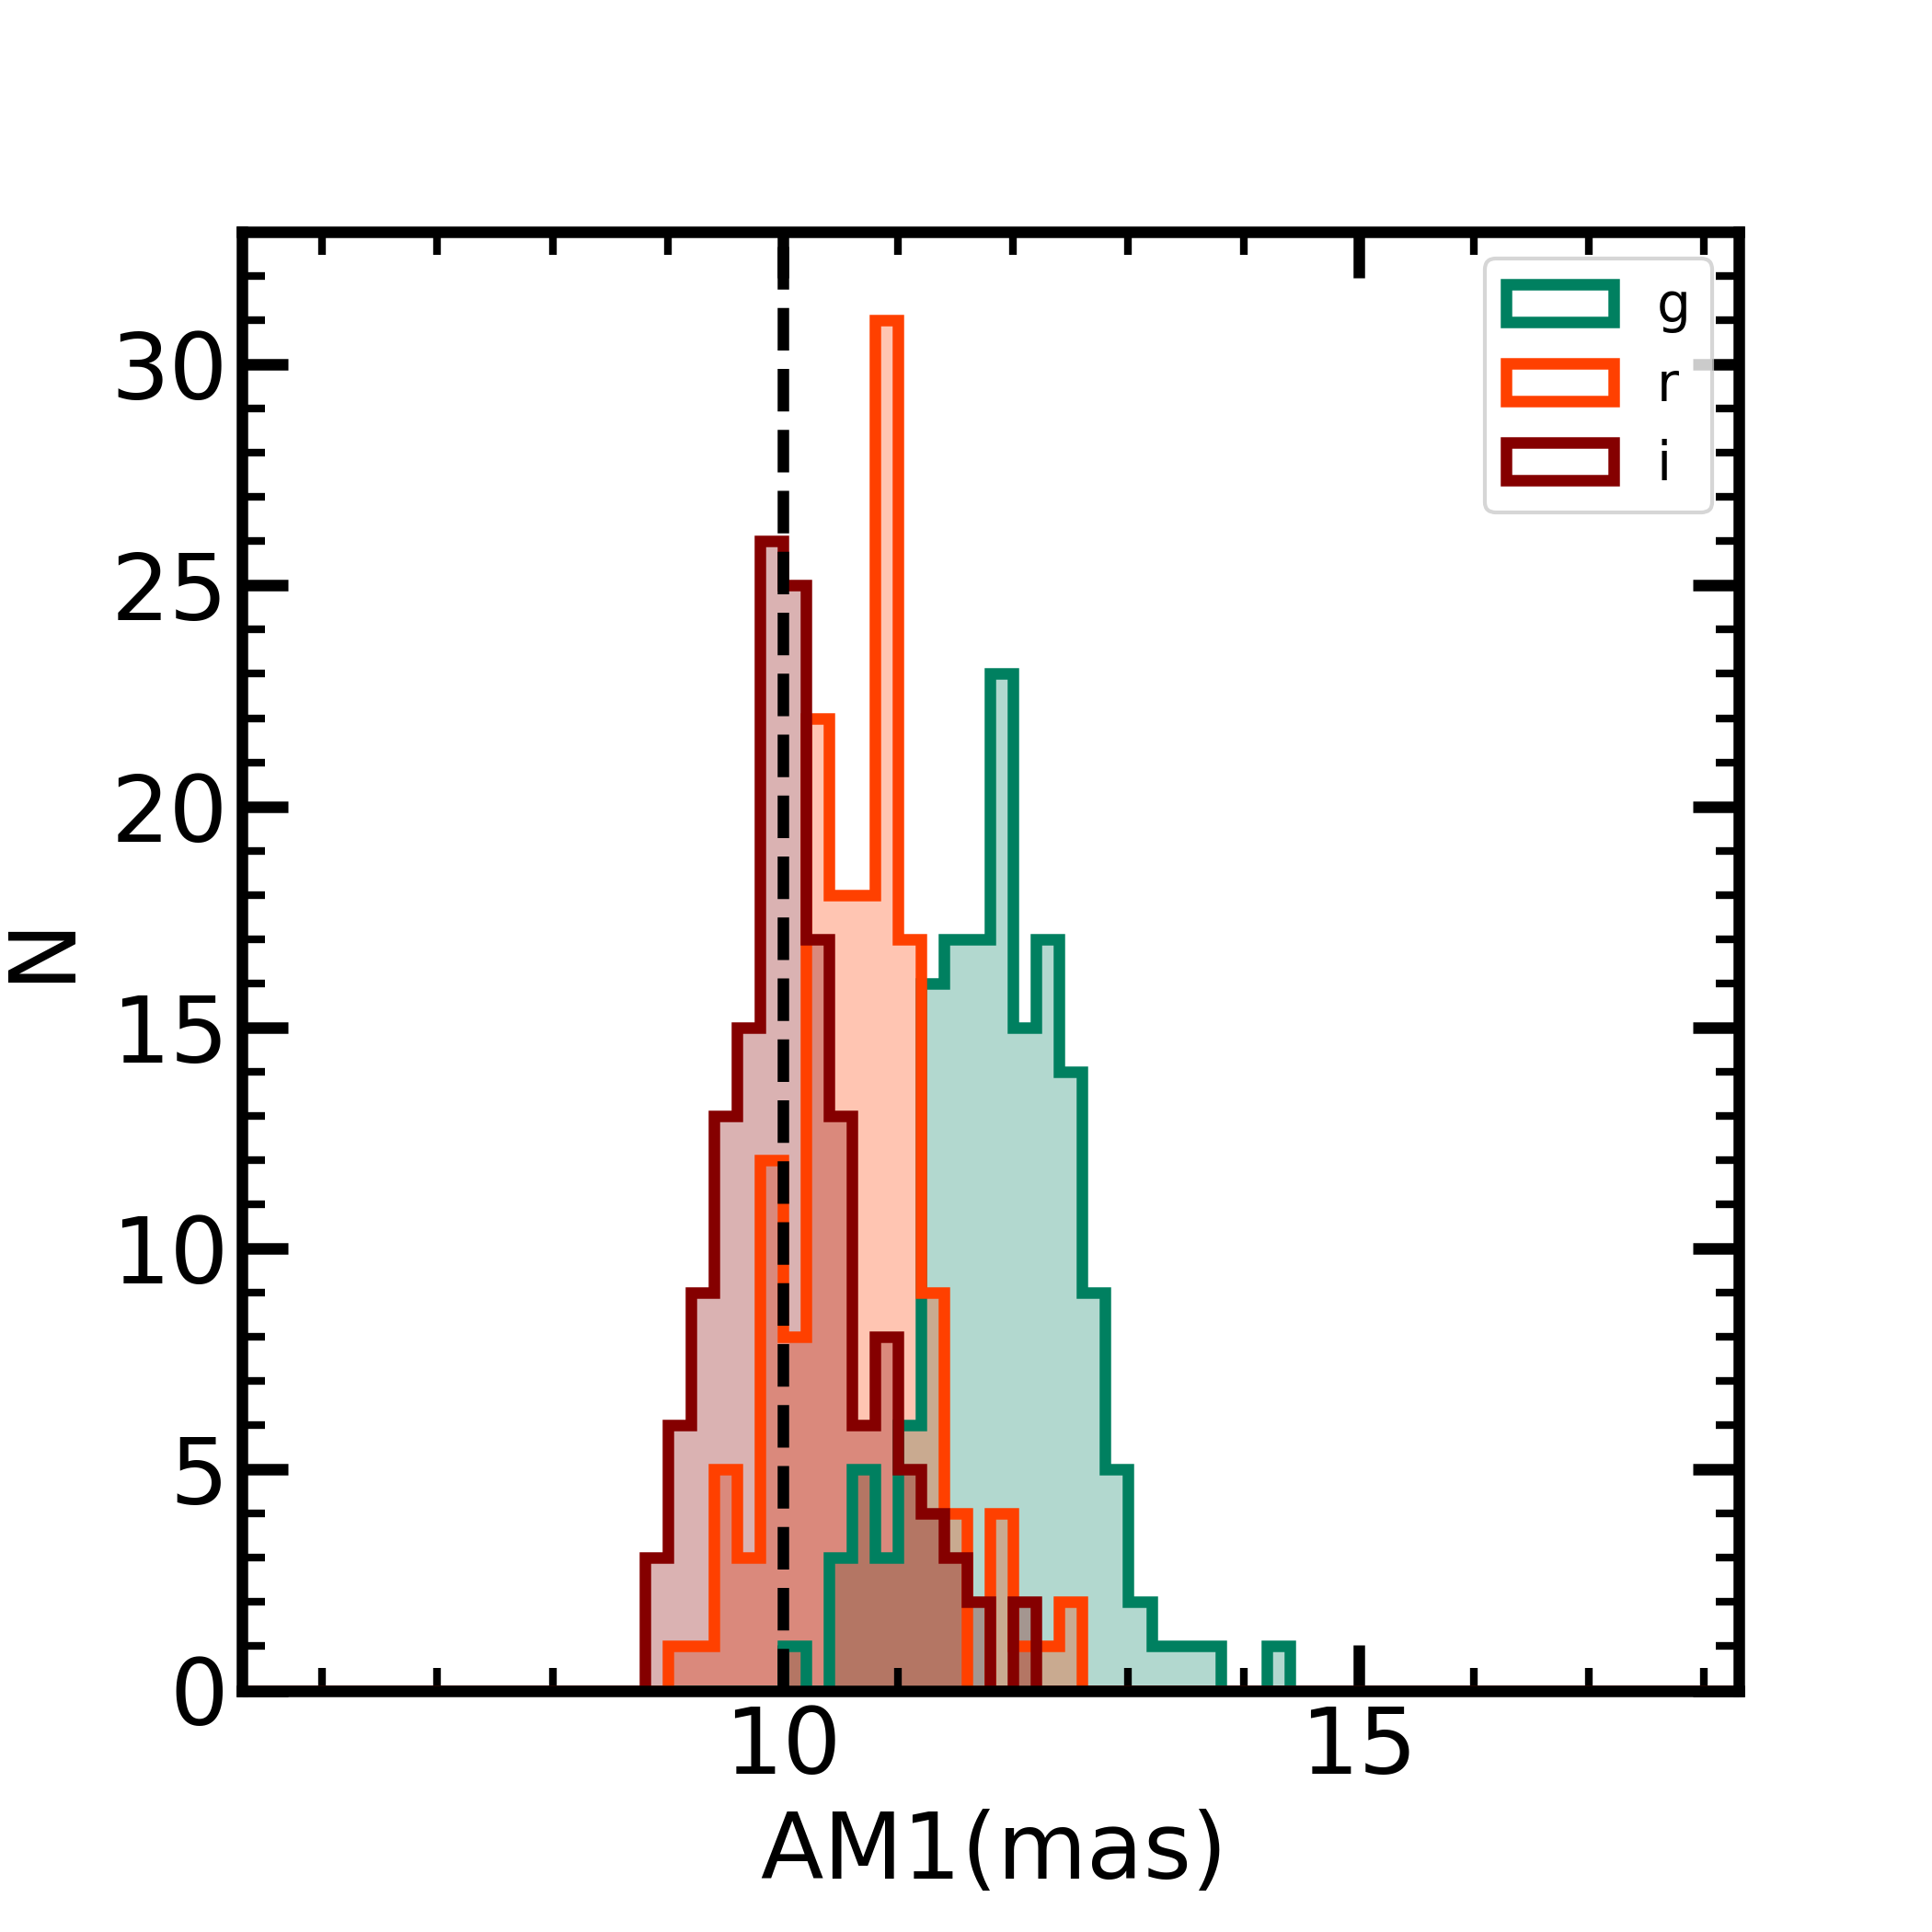
\includegraphics[width=0.98\textwidth]{figures/dp02_am1_alltracts_gri}
\end{subfigure}%
\begin{subfigure}{.5\textwidth}
    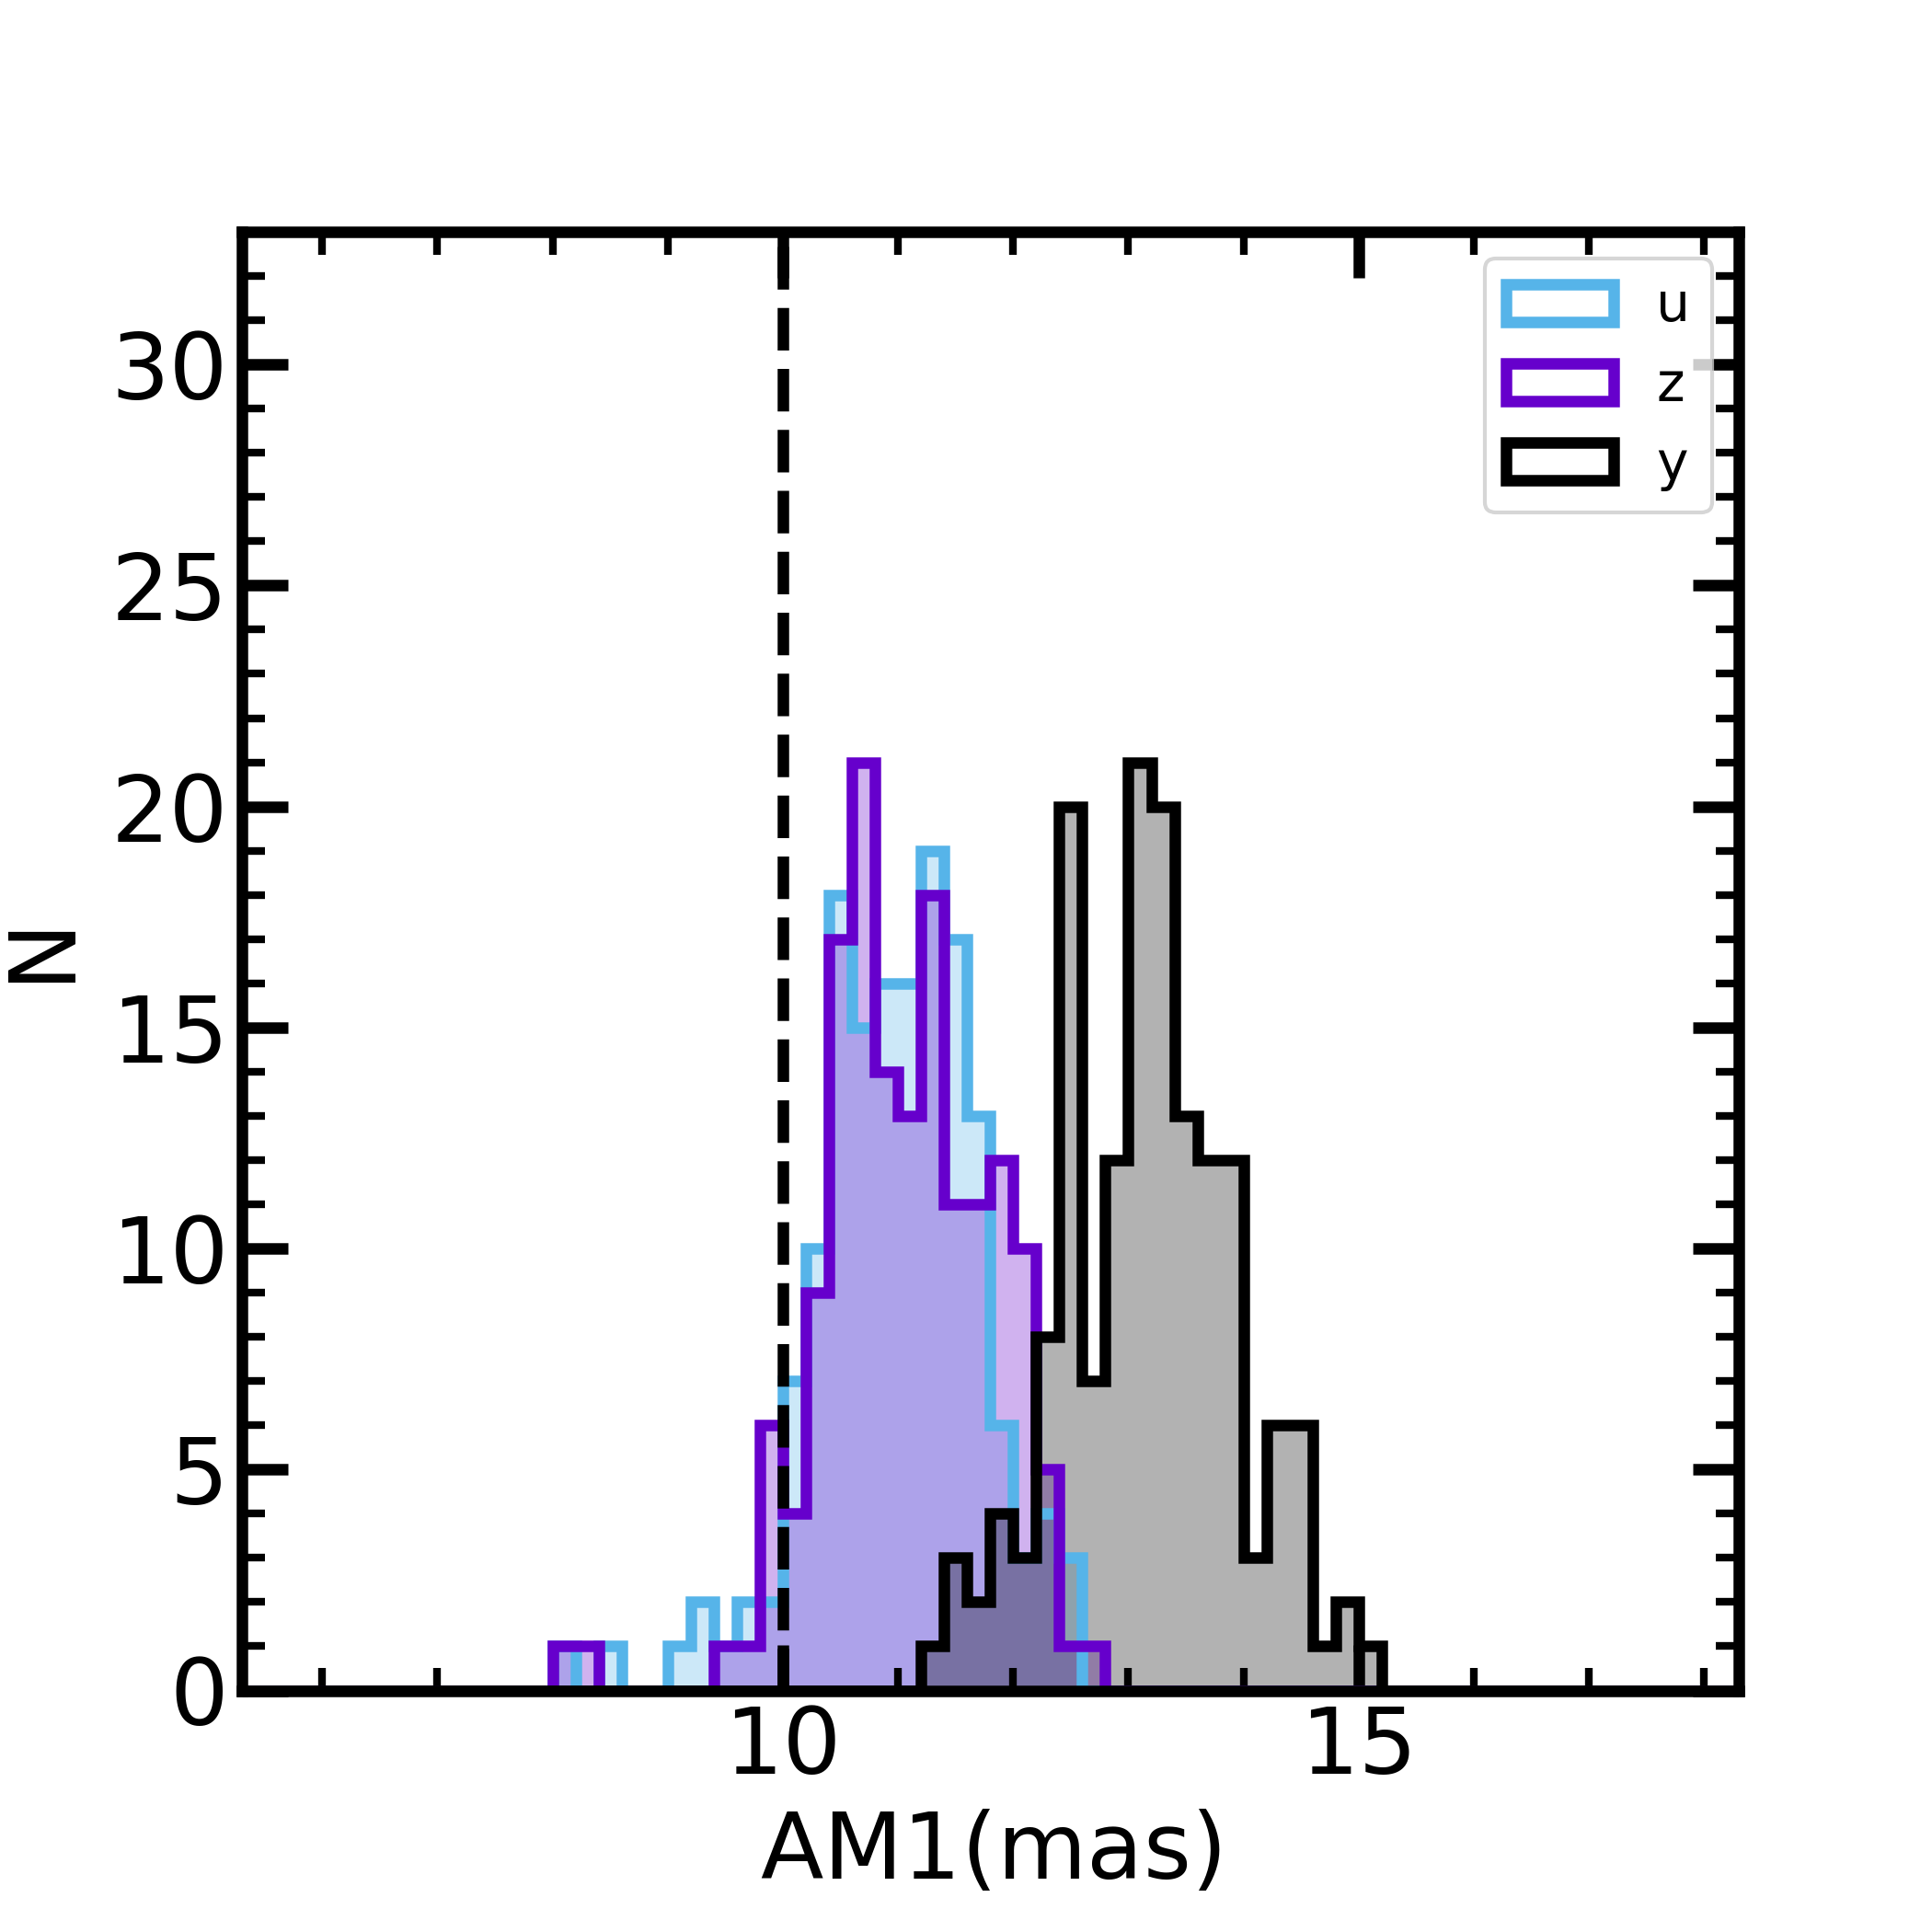
\includegraphics[width=0.98\textwidth]{figures/dp02_am1_alltracts_uzy}
\end{subfigure}
\begin{subfigure}{.5\textwidth}
    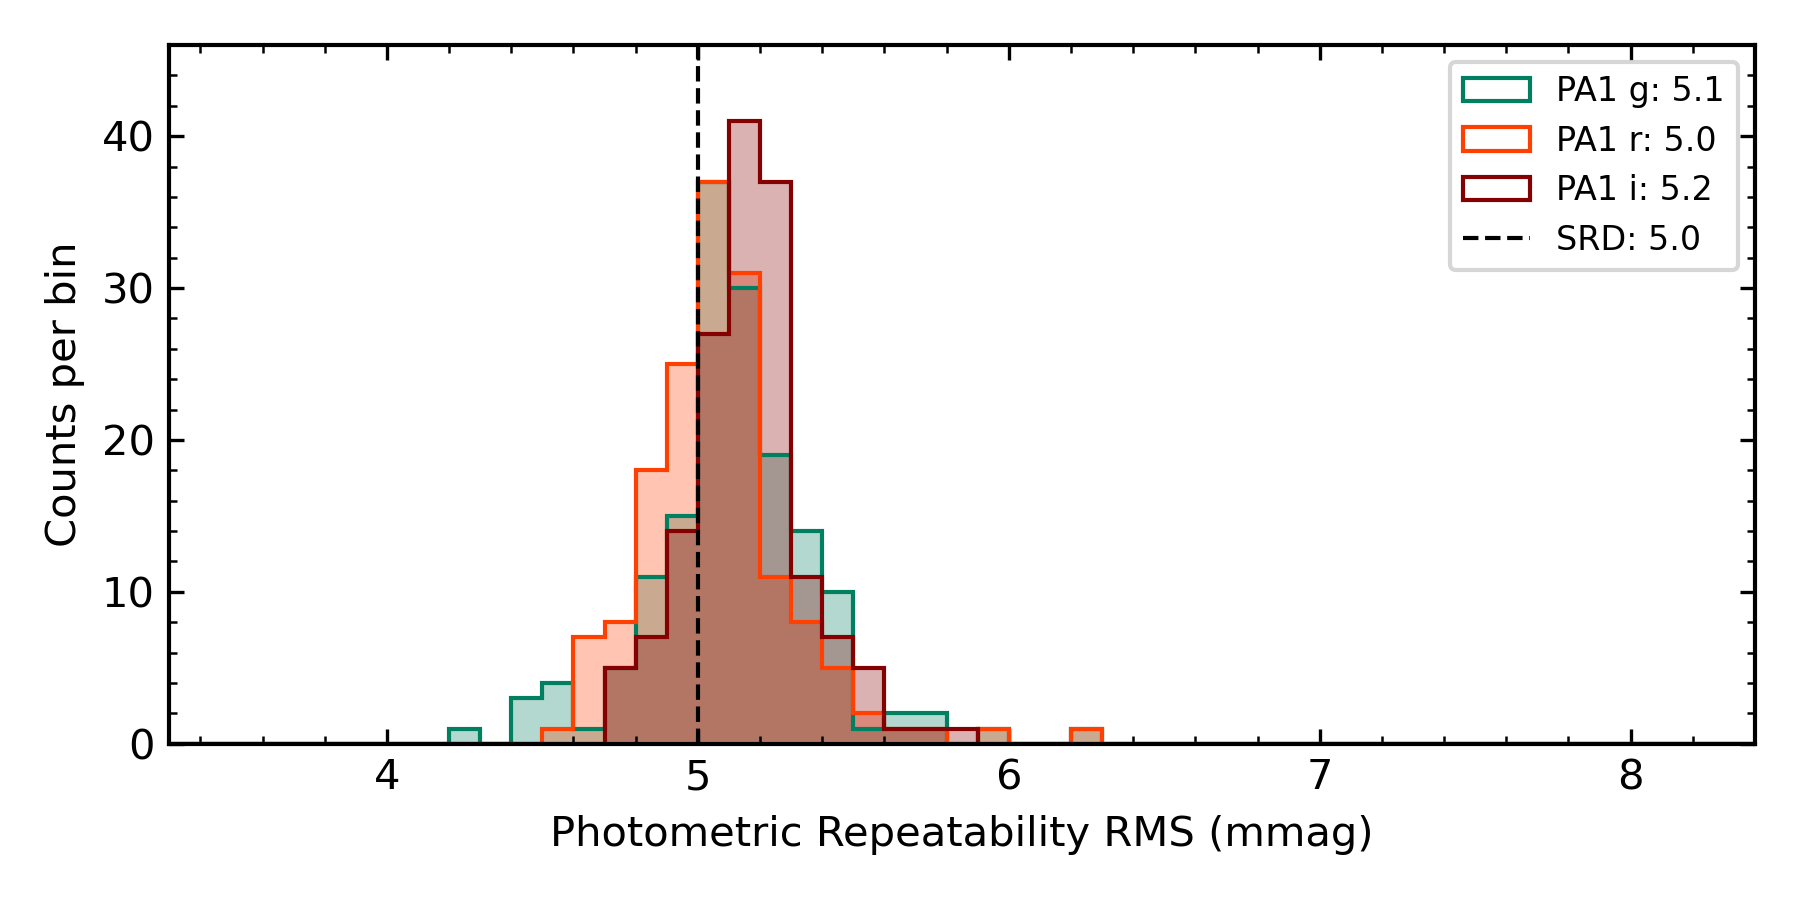
\includegraphics[width=0.98\textwidth]{figures/dp02_pa1_alltracts_gri}
\end{subfigure}%
\begin{subfigure}{.5\textwidth}
    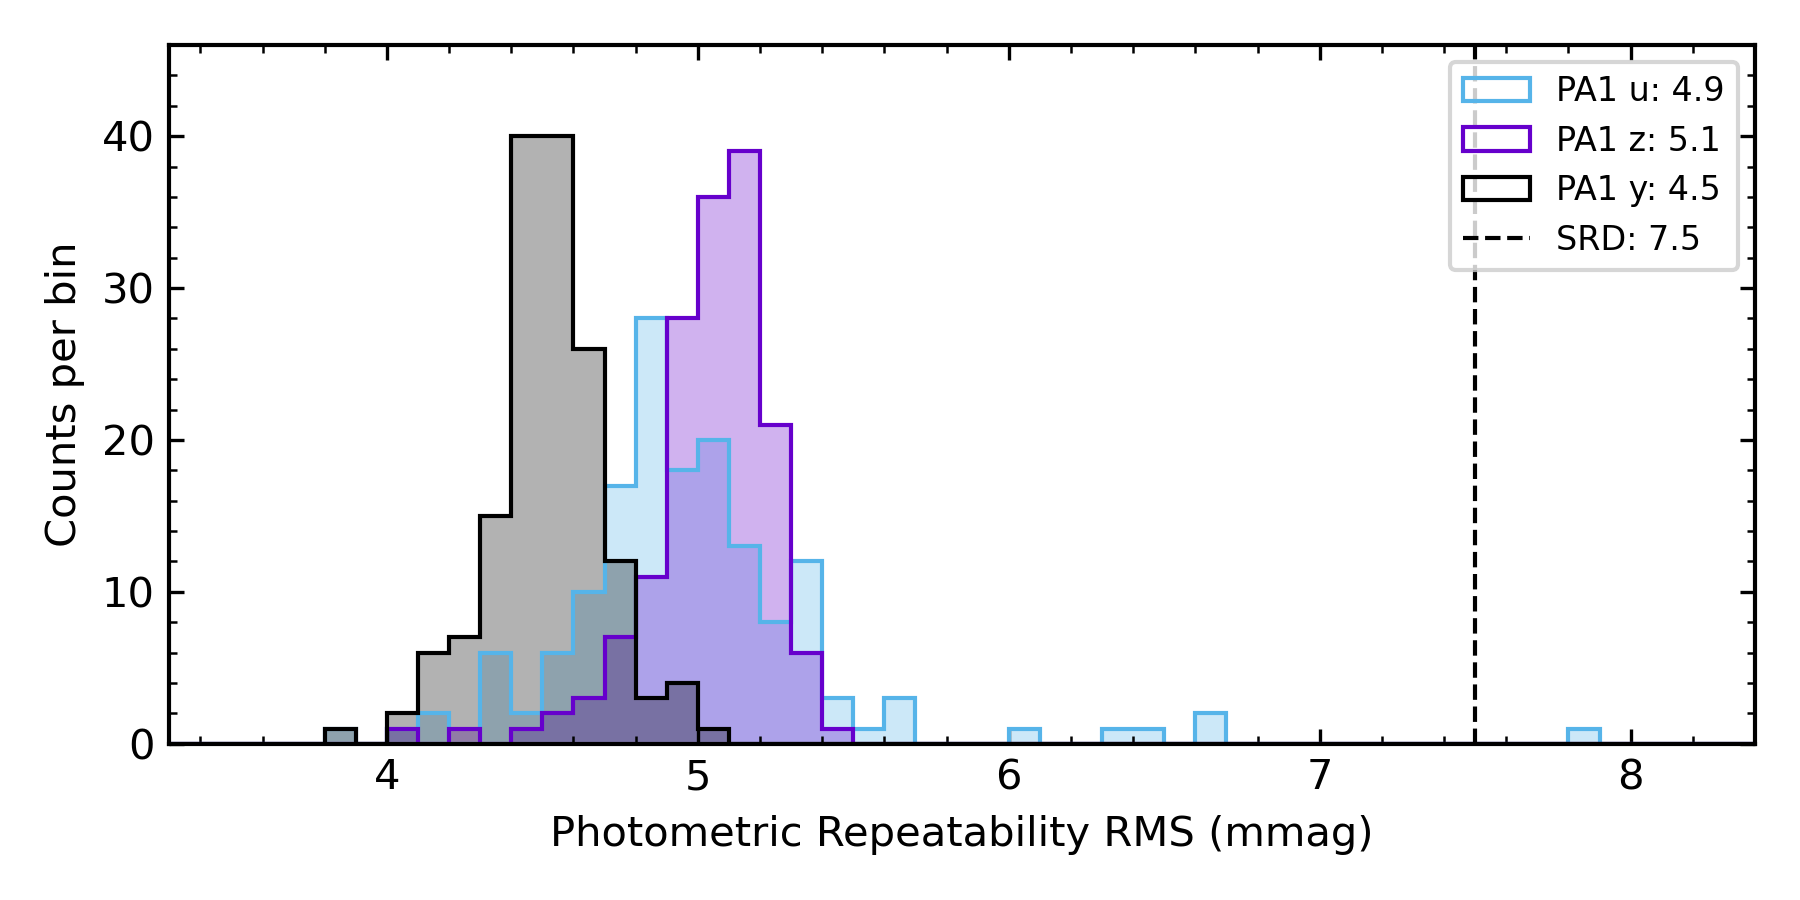
\includegraphics[width=0.98\textwidth]{figures/dp02_pa1_alltracts_uzy}
\end{subfigure}
\par\medskip % force a bit of vertical whitespace
\caption[short]{Distributions of per-visit and per object metrics computed as part of the DP0.2 reprocessing and (b) shows a focal plane image with computed metrics overlayed Show object level and source level }
\label{fig:faro_dp02_distr}
\end{figure}

\section{Current Status and Future Development} \label{sec:future}

The \faro framework is released as part of the LSST Science Pipelines distribution and is running in 
nightly and weekly CI builds on small representative CI datasets and on a a few tracts of HSC and DESC DC2 data to track the performance of the LSST Science Pipelines. 
\faro is used to produce a detailed Characterization Metric Report for major 6-monthly releases of the pipelines. 
\faro is starting to be used to characterize the performance of preliminary data from the Rubin Auxiliary Telescope imaging campaigns and was successfully run as at scale on the outputs of the Rubin Operations Data Preview 0.2 processing of the DESC DC2 300 \degsq dataset.
A large number of the LSST SRD metrics have been implemented in \faro spanning a range of analysis contexts; a near term focus will be on completing the implementation of these normative science performance metrics. 
A next goal will be a strong focus on the needs of LSST commissioning and to support the implementation of ad-hoc metrics to understand the performance of the as-built system, in particular to provide near real-time feedback and monitoring of the quality of data taken on the mountain. 
One indicator of the success of \faro is the steadily increasing number of active developers defining and implementing metics to characterize and diagnose performance and issues 

\section{Conclusions} \label{sec:conclusions}

In this paper, we have presented \faro, the LSST framework for automatically computing scalar performance metrics on the outputs of the LSST science pipelines. 
and shown how defining and tracking science performance  metrics.
We show that the development of an framework for the automated computation of metrics on a range of spatial and temporal scales makes this task easy and is critical to gain rapid insight into the performance of the developing system and address issues in a time manner and to help us to rapidly identify where to focus efforts of investigation to resolve and debug issues. 
In addition to computing the normative science performance metrics on the LSST data products, \faro provides a flexible and easy-to-use framework in which anyone can define and write a metric that will be computed on the LSST data products and run as part of the LSST science pipelines. 
The system is successfully running in nightly and weekly CI on precursor datasets to track the performance of the LSST science pipelines and provide regression analysis as development continues. 
\faro has also been successfully demonstrated at scale with the reprocessing of the DESC DC2 dataset \cite{2021ApJS..253...31L} at the Rubin Interim Data Facility (IDF) running on Google cloud \cite{2021arXiv211115030O} in the context of Rubin Data Preview 0.2 (DP0.2)\cite{RTN-001}. 
As we enter LSST commissioning, \faro will be a powerful tool to gain rapid insight into the quality of the data coming off the telescope. 
